\chapter{Start Here}
\label{cha:基础操作}

\section{Power On}

Before powering on the robot, please reconfirm that you have read \prettyref{sec:安全指南} and are now following it to eliminate potential risks and ensure safe operation.

\begin{figure}[hb]
    \centering
    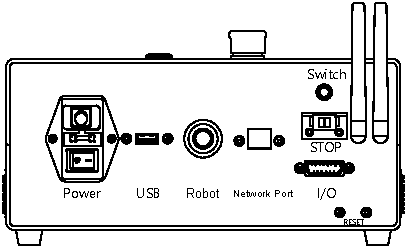
\includegraphics[height=5cm]{en/image/robot_control_box_back.pdf}
    \caption{Schematic diagram of the control box back panel}
    \label{fig:控制箱背板示意图}
\end{figure}

\begin{enumerate}
\item Put the robot cable into the ``Robot'' port of the control box.
\item Plug the power cord into the control box and connect the power plug to the 220$\unit{V}$ AC outlet.
\item Ensure that the emergency stop button on the top of the control box is in the released\footnote{When the emergency stop button is pop-up, it is in the released state. Conversely, when it is pressed, it is in the locked state.} state.
\item Turn on the red main power switch on the back panel of the control box, and the switch indicator light is on.
\item Long press (for about 3 seconds) the switch button on the top of the control box or the external switch button (optional) until the indicator light of the switch button on the top of the control box turns blue. Wait for the light on the shoulder of the robot comes up to mark the complete of the power­on operation of the control box and the robot.
\end{enumerate}

    %  \footnotetext[a]{当使用$100\sim 200\unit{V}$ 供电时}
    %  \footnotetext[b]{当使用$200\sim 240\unit{V}$ 供电时}
\danger{\begin{itemize}
\item Make sure that the power strip of the control box is well grounded.
\item Make sure that the input current of the control box power supply is protected by the leakage protection device and the appropriate overcurrent protection device.
\item Make sure that all cables are properly connected before the control box is powered on, and always use the original power cord correctly.
\end{itemize}}

\danger[WARNING] {\begin{itemize}
\item It is forbidden to disconnect or pull the robot cable when the robot is started.
\item Do not extend or modify the robot cable.
\item Do not damage the power cord or place heavy objects on the power cord.
\item Do not use damaged or non­compliant outlets.
\item Do not allow dust or mill scales to adhere to the power plug and socket.
\end{itemize}}

% \clearpage

\section{Connect to the Robot}
LM3 supports both wired network connection and wireless network connection. The wireless network connection currently only supports access to the Wi­Fi hotspot network integrated in the control box.
\subsection{Wired Network Connection}

Use a network cable to connect the network port on the back panel of the control box with the LAN port of the router or switch, and ensure that the computer, tablet, mobile phone or other graphical terminal device used to operate the robot is connected to the same network as the robot.

The connection diagram of the wired network is shown in \prettyref{fig:有线网络连接拓扑图}:

\begin{figure}[ht]
    \centering
    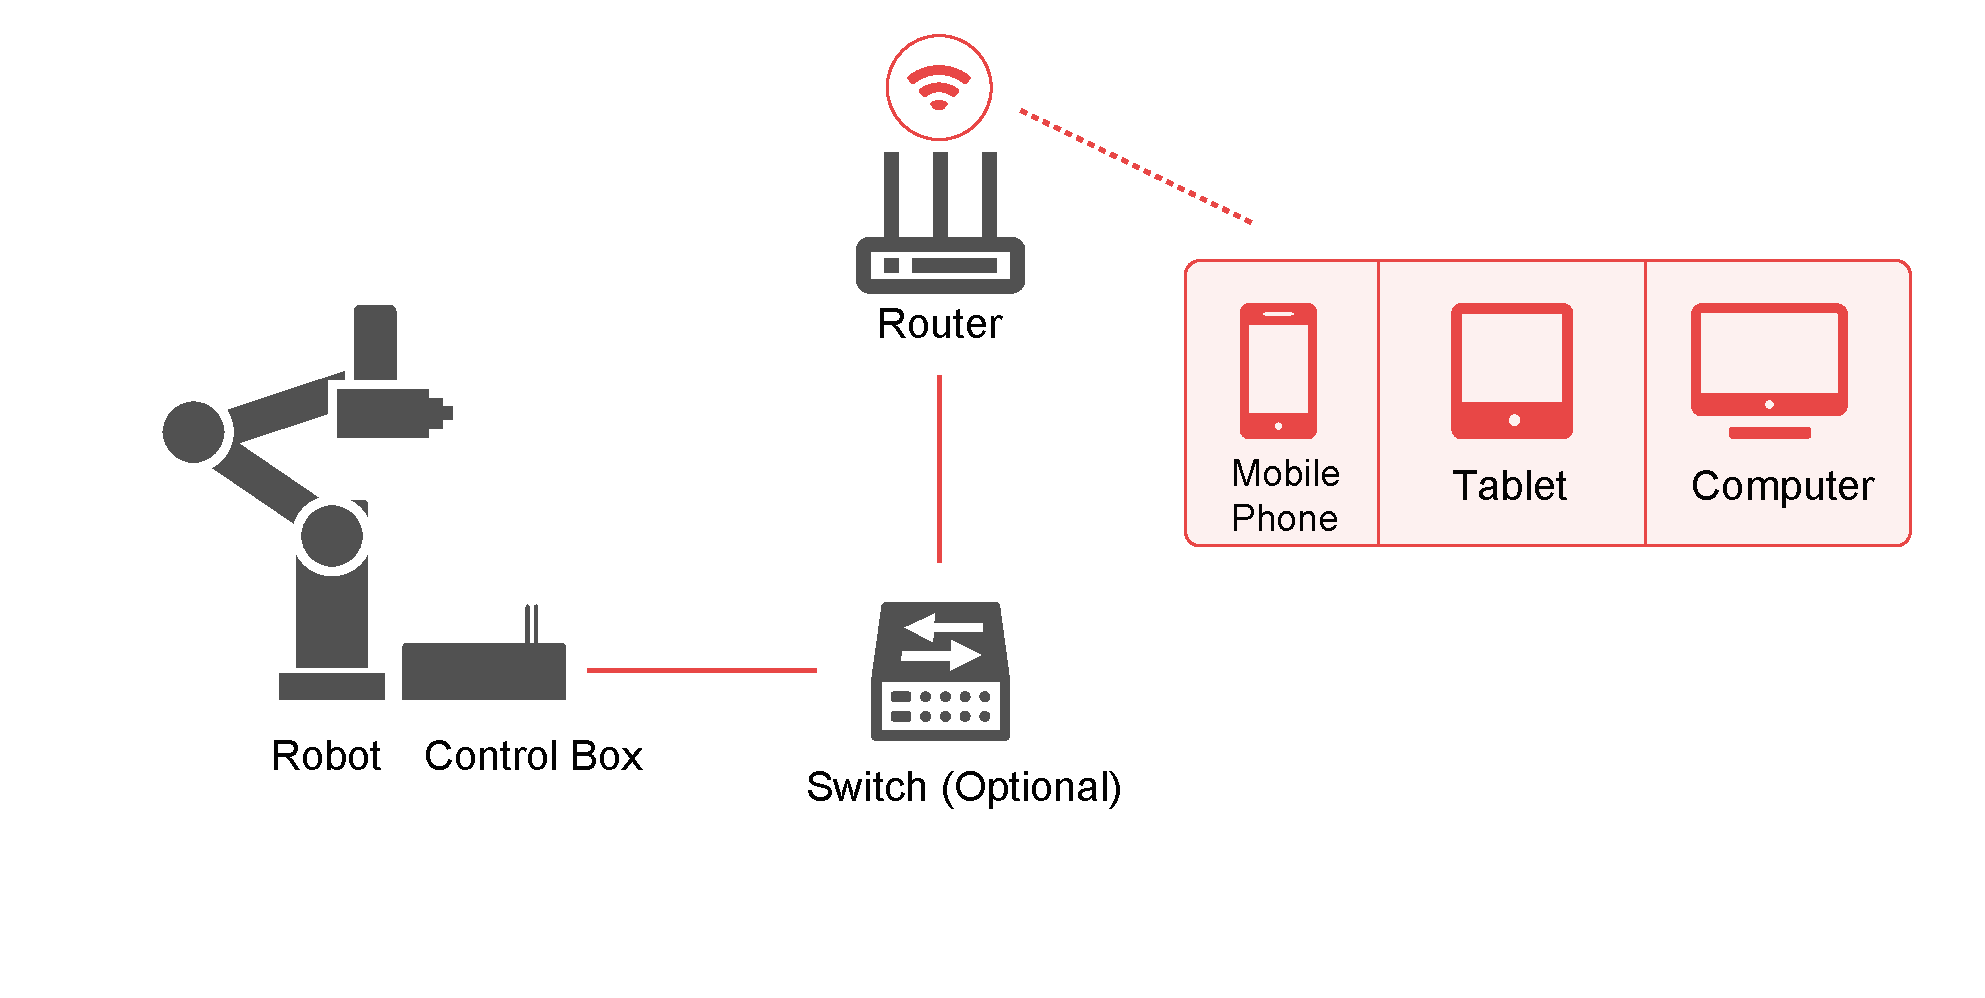
\includegraphics[width=\textwidth]{image/network-1.pdf}
    \caption{Wired network connection topology diagram}
	\label{fig:有线网络连接拓扑图}

    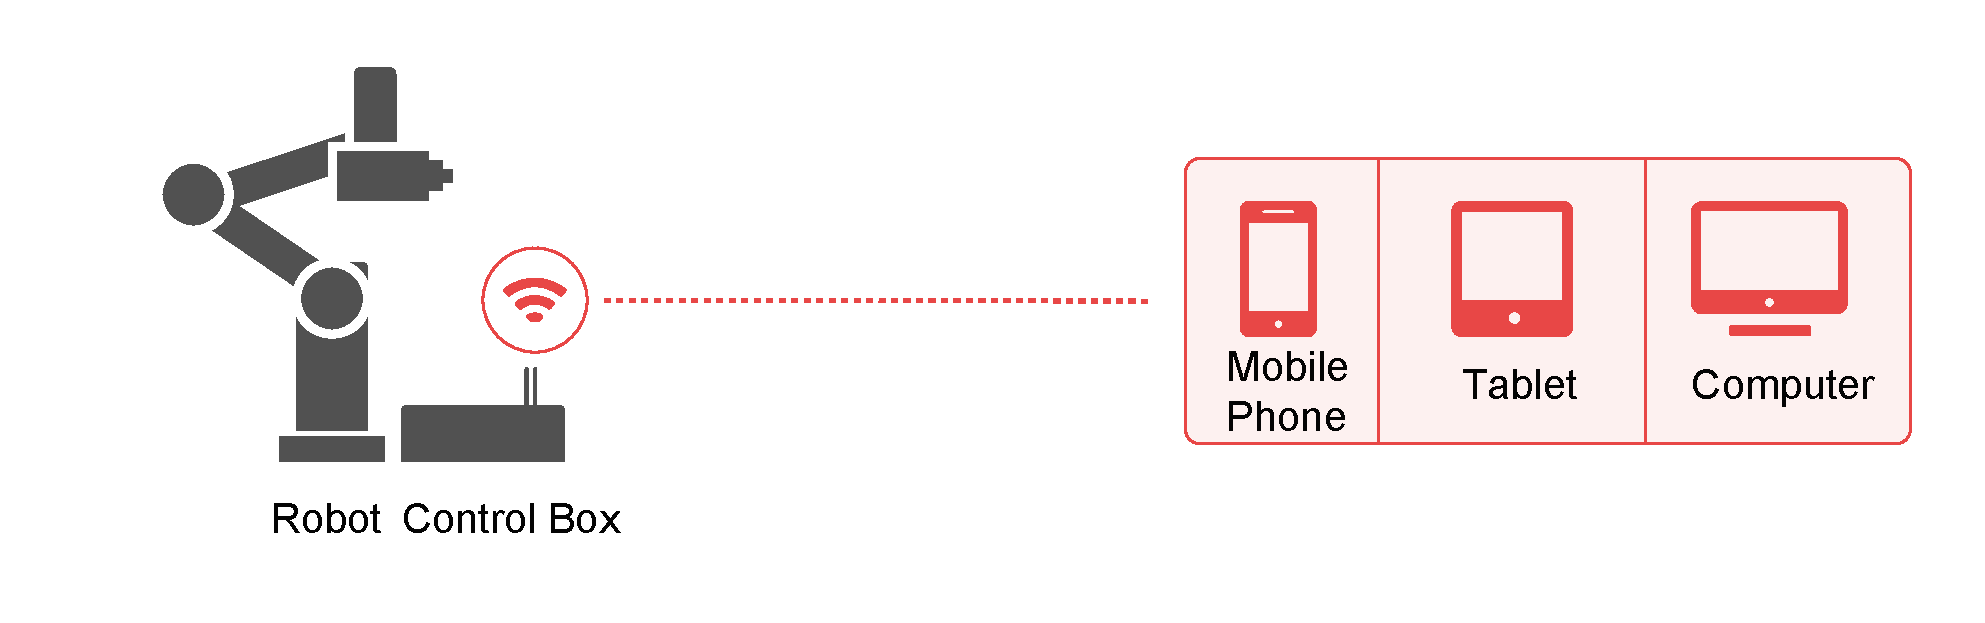
\includegraphics[width=\textwidth]{image/network-2.pdf}
    \caption{Wireless network connection topology diagram}
    \label{fig:无线网络连接拓扑图}
\end{figure}

% \clearpage

\subsection{Wireless Network Connection}
After the robot leaves the factory, a Wi­Fi hotspot with a name same as the device name\footnote{The device name can be found on the nameplate of the control box.} will be enabled by default. The format of the device name is \verb|Lebai-123456| (the last 6 digits are random characters), and the default password is \verb|88888888| (eight ``8''s). You can connect to the Wi­Fi hotspot network corresponding to the device name through the Wi­Fi function of a computer, tablet, mobile phone or other graphical terminal device to connect and control the robot.

% \begin{figure}[ht]
%     \centering
% \end{figure}

% \clearpage

\section{Login to \LM}
Learning the operation of the \LM\ system will help you to use our robot products more conveniently and quickly. 
Open a browser on your computer, tablet, mobile phone or other graphical terminal device and enter the following address in the address bar:
\begin{itemize}
	\item If you use a wired network: \url{http://<IP>}\footnote{The wired network address can be viewed in the device list on the router page of the connected network. The viewing method varies according to the brand and type of the device. For the specific viewing method, please refer to the router device manual or contact the corresponding device manufacturer.}
	\item If you use a wireless hotspot: \url{http://10.20.17.1}
\end{itemize}

After loading, you will enter the login page. Please enter the default code: \verb|1111|, then click \btn{LOGIN} or press \kbd{Enter}.

\begin{figure}[ht]
    \centering
    
\includegraphics[height=3.4cm]{en/image/2-4.png}
    \caption{Login to \LM}
    \label{fig:登录LM}
\end{figure}

\clearpage

\section{Welcome Screen}

To login to \LM for the first time after the robot is unpacked and powered on, first, you need to follow the instructions on the setup guide page to set up the robot before initial use.
\subsection{System Settings}
The first step is to customize the language, time zone, and time in \mnu{System Settings}.

\begin{figure}[ht]
    \centering
    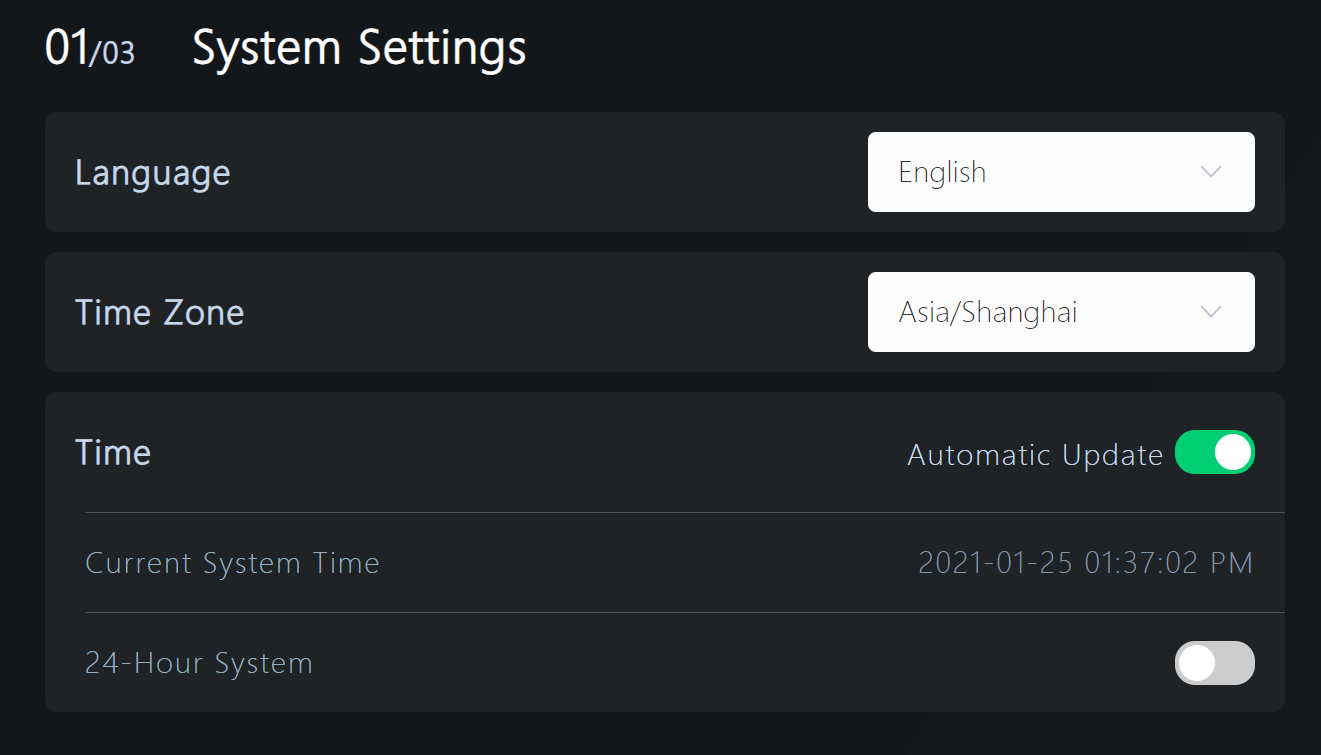
\includegraphics[width=\textwidth]{en/image/2-5.png}
    \caption{System Settings}
    \label{fig:系统设置}
\end{figure}

\subsection{Robot Settings}
The second step is to set the robot installation mode, operation mode and collision detection in \mnu{Robot Settings}.
\begin{enumerate}
\item Installation

	According to the actual install direction, refer to the \\\mnu{Icon comparison table} in \prettyref{fig:安装方式} to choose up, down, or side installation.

	\begin{figure}[ht]
		\centering
		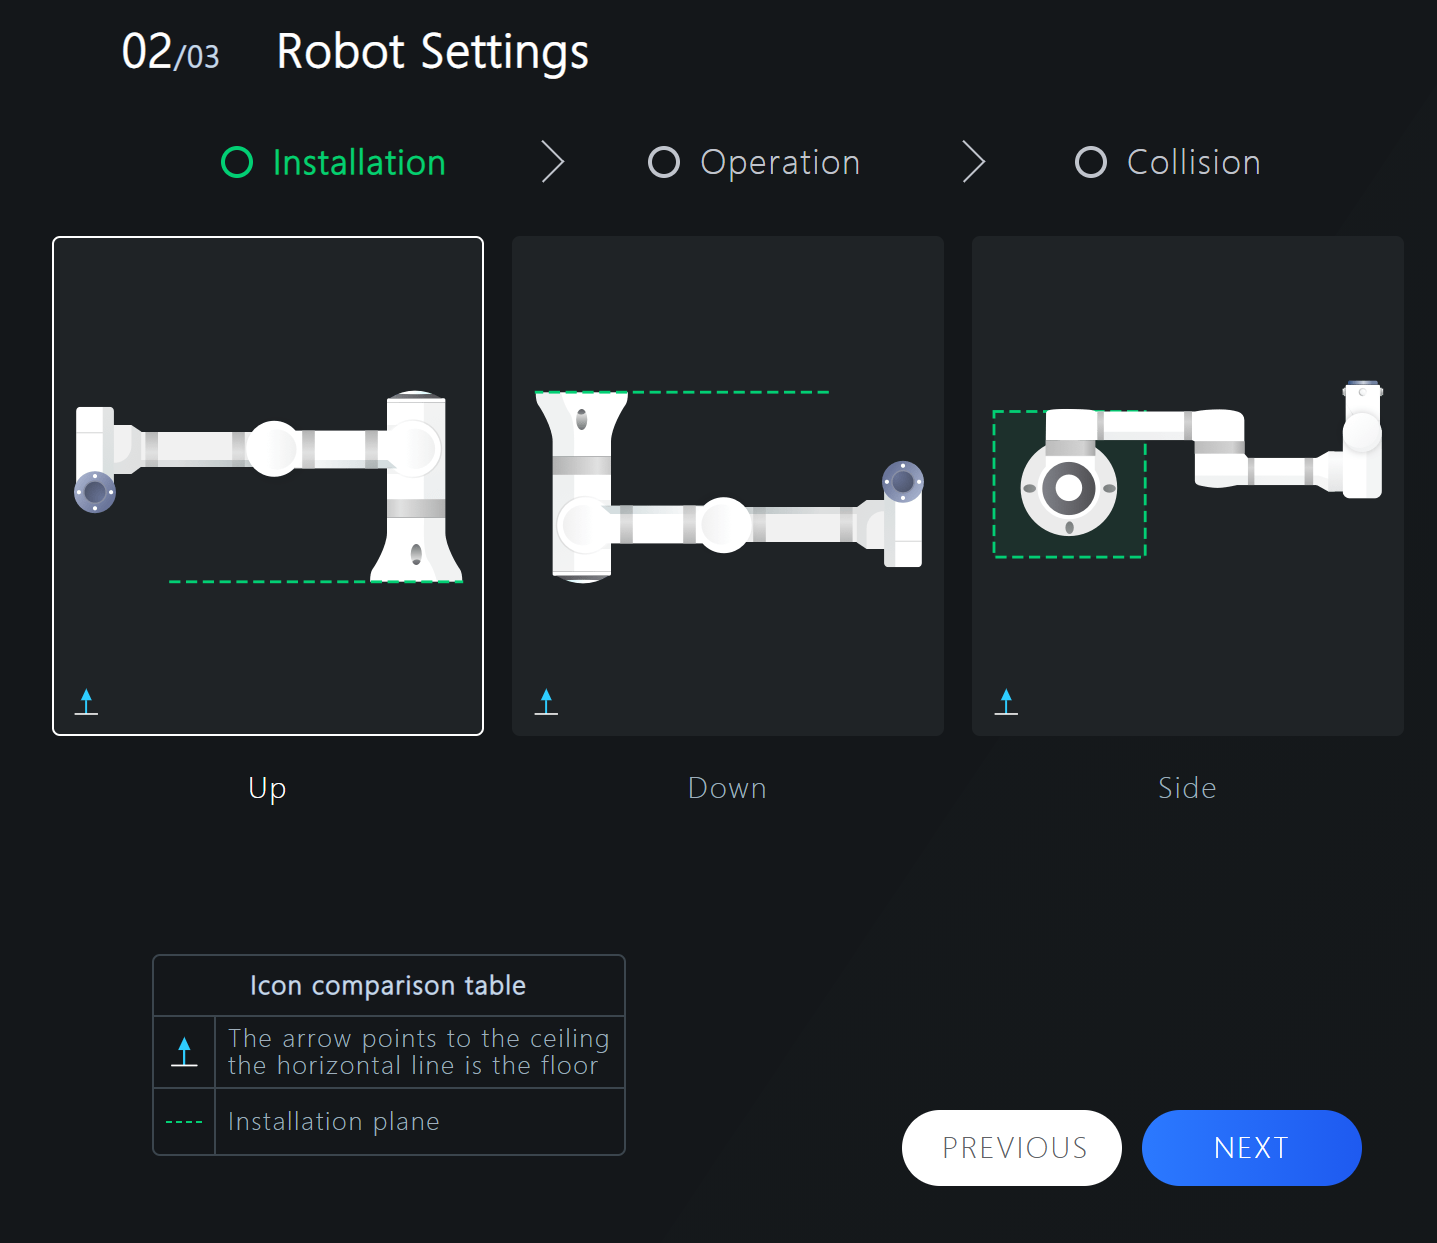
\includegraphics[width=\textwidth]{en/image/2-6.png}
		\caption{Install direction}
		\label{fig:安装方式}
	\end{figure}

	\danger{The choice of install direction must be consistent with the actual install direction, otherwise it may cause accidental injury.}

% \clearpage

\item Operation

	You can choose between the \mnu{Normal Mode} and \mnu{Expert Mode}.
	
	The \mnu{Normal Mode} is suitable for novices who have no programming basics, thus there is no need to understand any logic or codes. The \mnu{Expert Mode} is suitable for advanced users who have some basic knowledge in programming and logic. 

	You can choose the appropriate operation mode according to your own situation.

	\begin{figure}[ht]
		\centering
		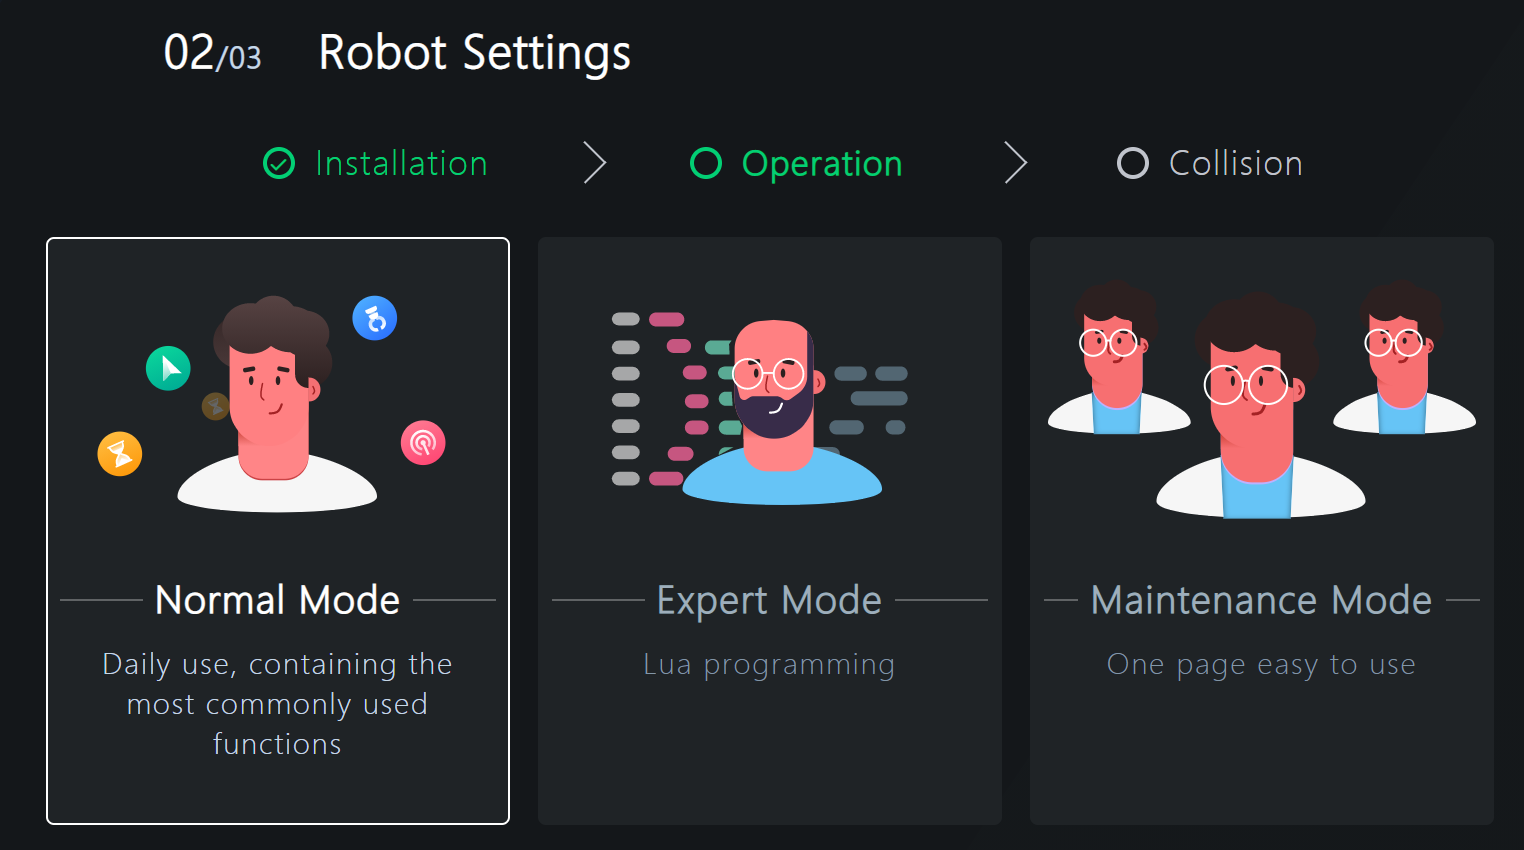
\includegraphics[width=\textwidth]{en/image/2-7.png}
		\caption{Operation mode}
		\label{fig:操作模式}
	\end{figure}

\clearpage

\item Collision

	The detection switch is on by default, and the \mnu{Action} is set to \mnu{Emergency Stop} by default. You can choose between \\\mnu{Emergency Stop} or \mnu{Pause}, and you can drag the lever to adjust the \mnu{Detection Sensitivity}. Click \btn{NEXT} to enter the interface settings.

	\begin{figure}[ht]
		\centering
		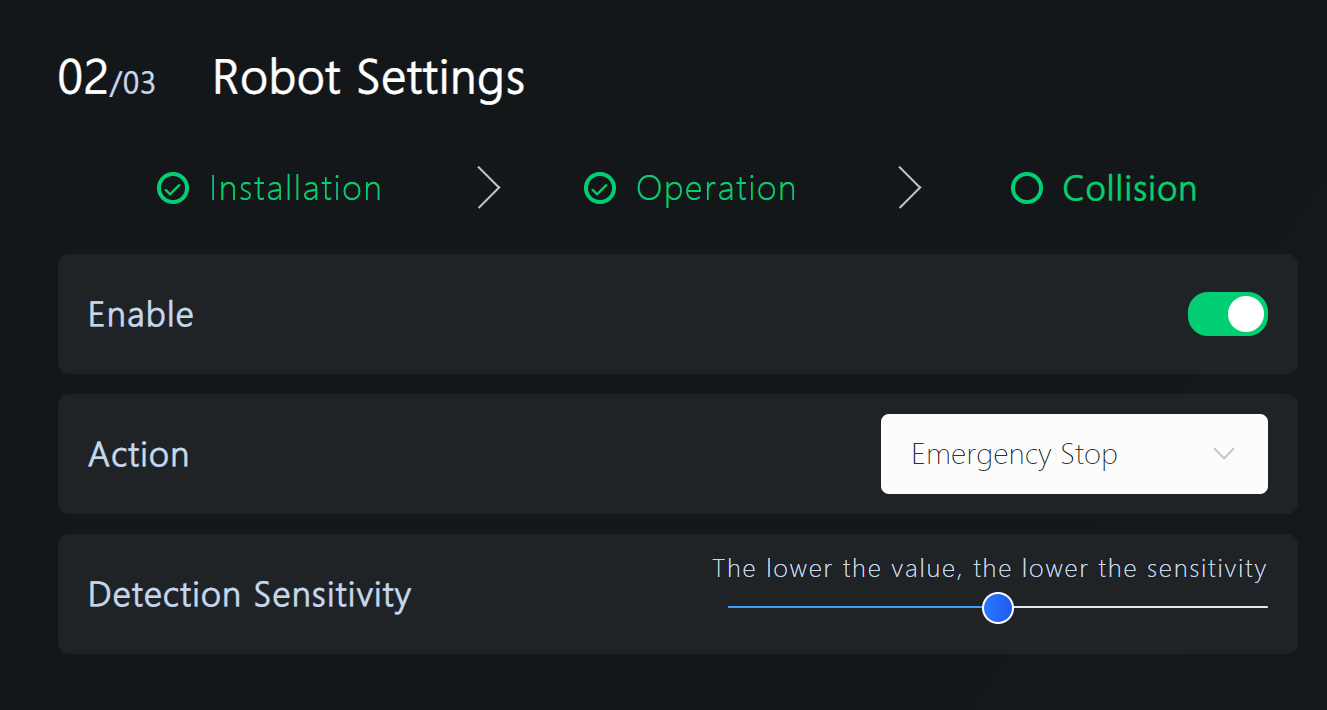
\includegraphics[width=\textwidth]{en/image/2-8.png}
		\caption{Collision detection}
		\label{fig:碰撞检测}
	\end{figure}

	\danger{When the robot is operating, no matter whether the collision detection function is turned on or not, it is forbidden to enter the robot's workspace\footnote{See \prettyref{sec:工作空间}.} without protection, otherwise there is a risk of personnel getting hit by the robot.}

\end{enumerate}

\clearpage

\subsection{Interface Settings}

The third step is to set the interface theme in the \mnu{Interface Settings}. It is recommended to use the \mnu{Dark theme}.
% 可以选择\mnu{深色主题}或\mnu{浅色主题},目前\LM 浅色主题还在测试阶段,

\begin{figure}[ht]
	\centering
	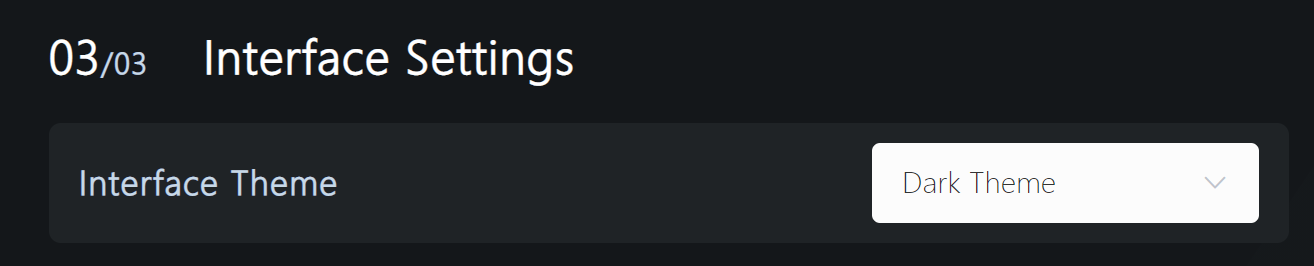
\includegraphics[width=\textwidth]{en/image/2-9.png}
	\caption{Interface Settings}
	\label{fig:界面设置}
\end{figure}

Click \btn{FINISH} to enter the home page of \LM.

% \clearpage

\section{Home}

The \LM homepage is divided into six areas: left panel, status area, control area, main function entrance, task history, and title bar at the top.

\newpage

\begin{itemize}
\item The left panel displays the robot temperature and joint temperature, the position and posture in the coordinate space, and the joint angle in the joint space.
\item The status area displays the real­time status of the robot.
\item The control area contains the robot's Start and Stop button, software Teaching buttons and Speed ratio adjustment controls.
\item The main function entrance contains three main function en­trances: \mnu{Scene}, \mnu{Control} and \mnu{Device}.
\item Task History contains a list of all task histories.
\item The right side of the top title bar contains Settings, Message Center and Logout.
\end{itemize}

\begin{figure}[ht]
	\centering
	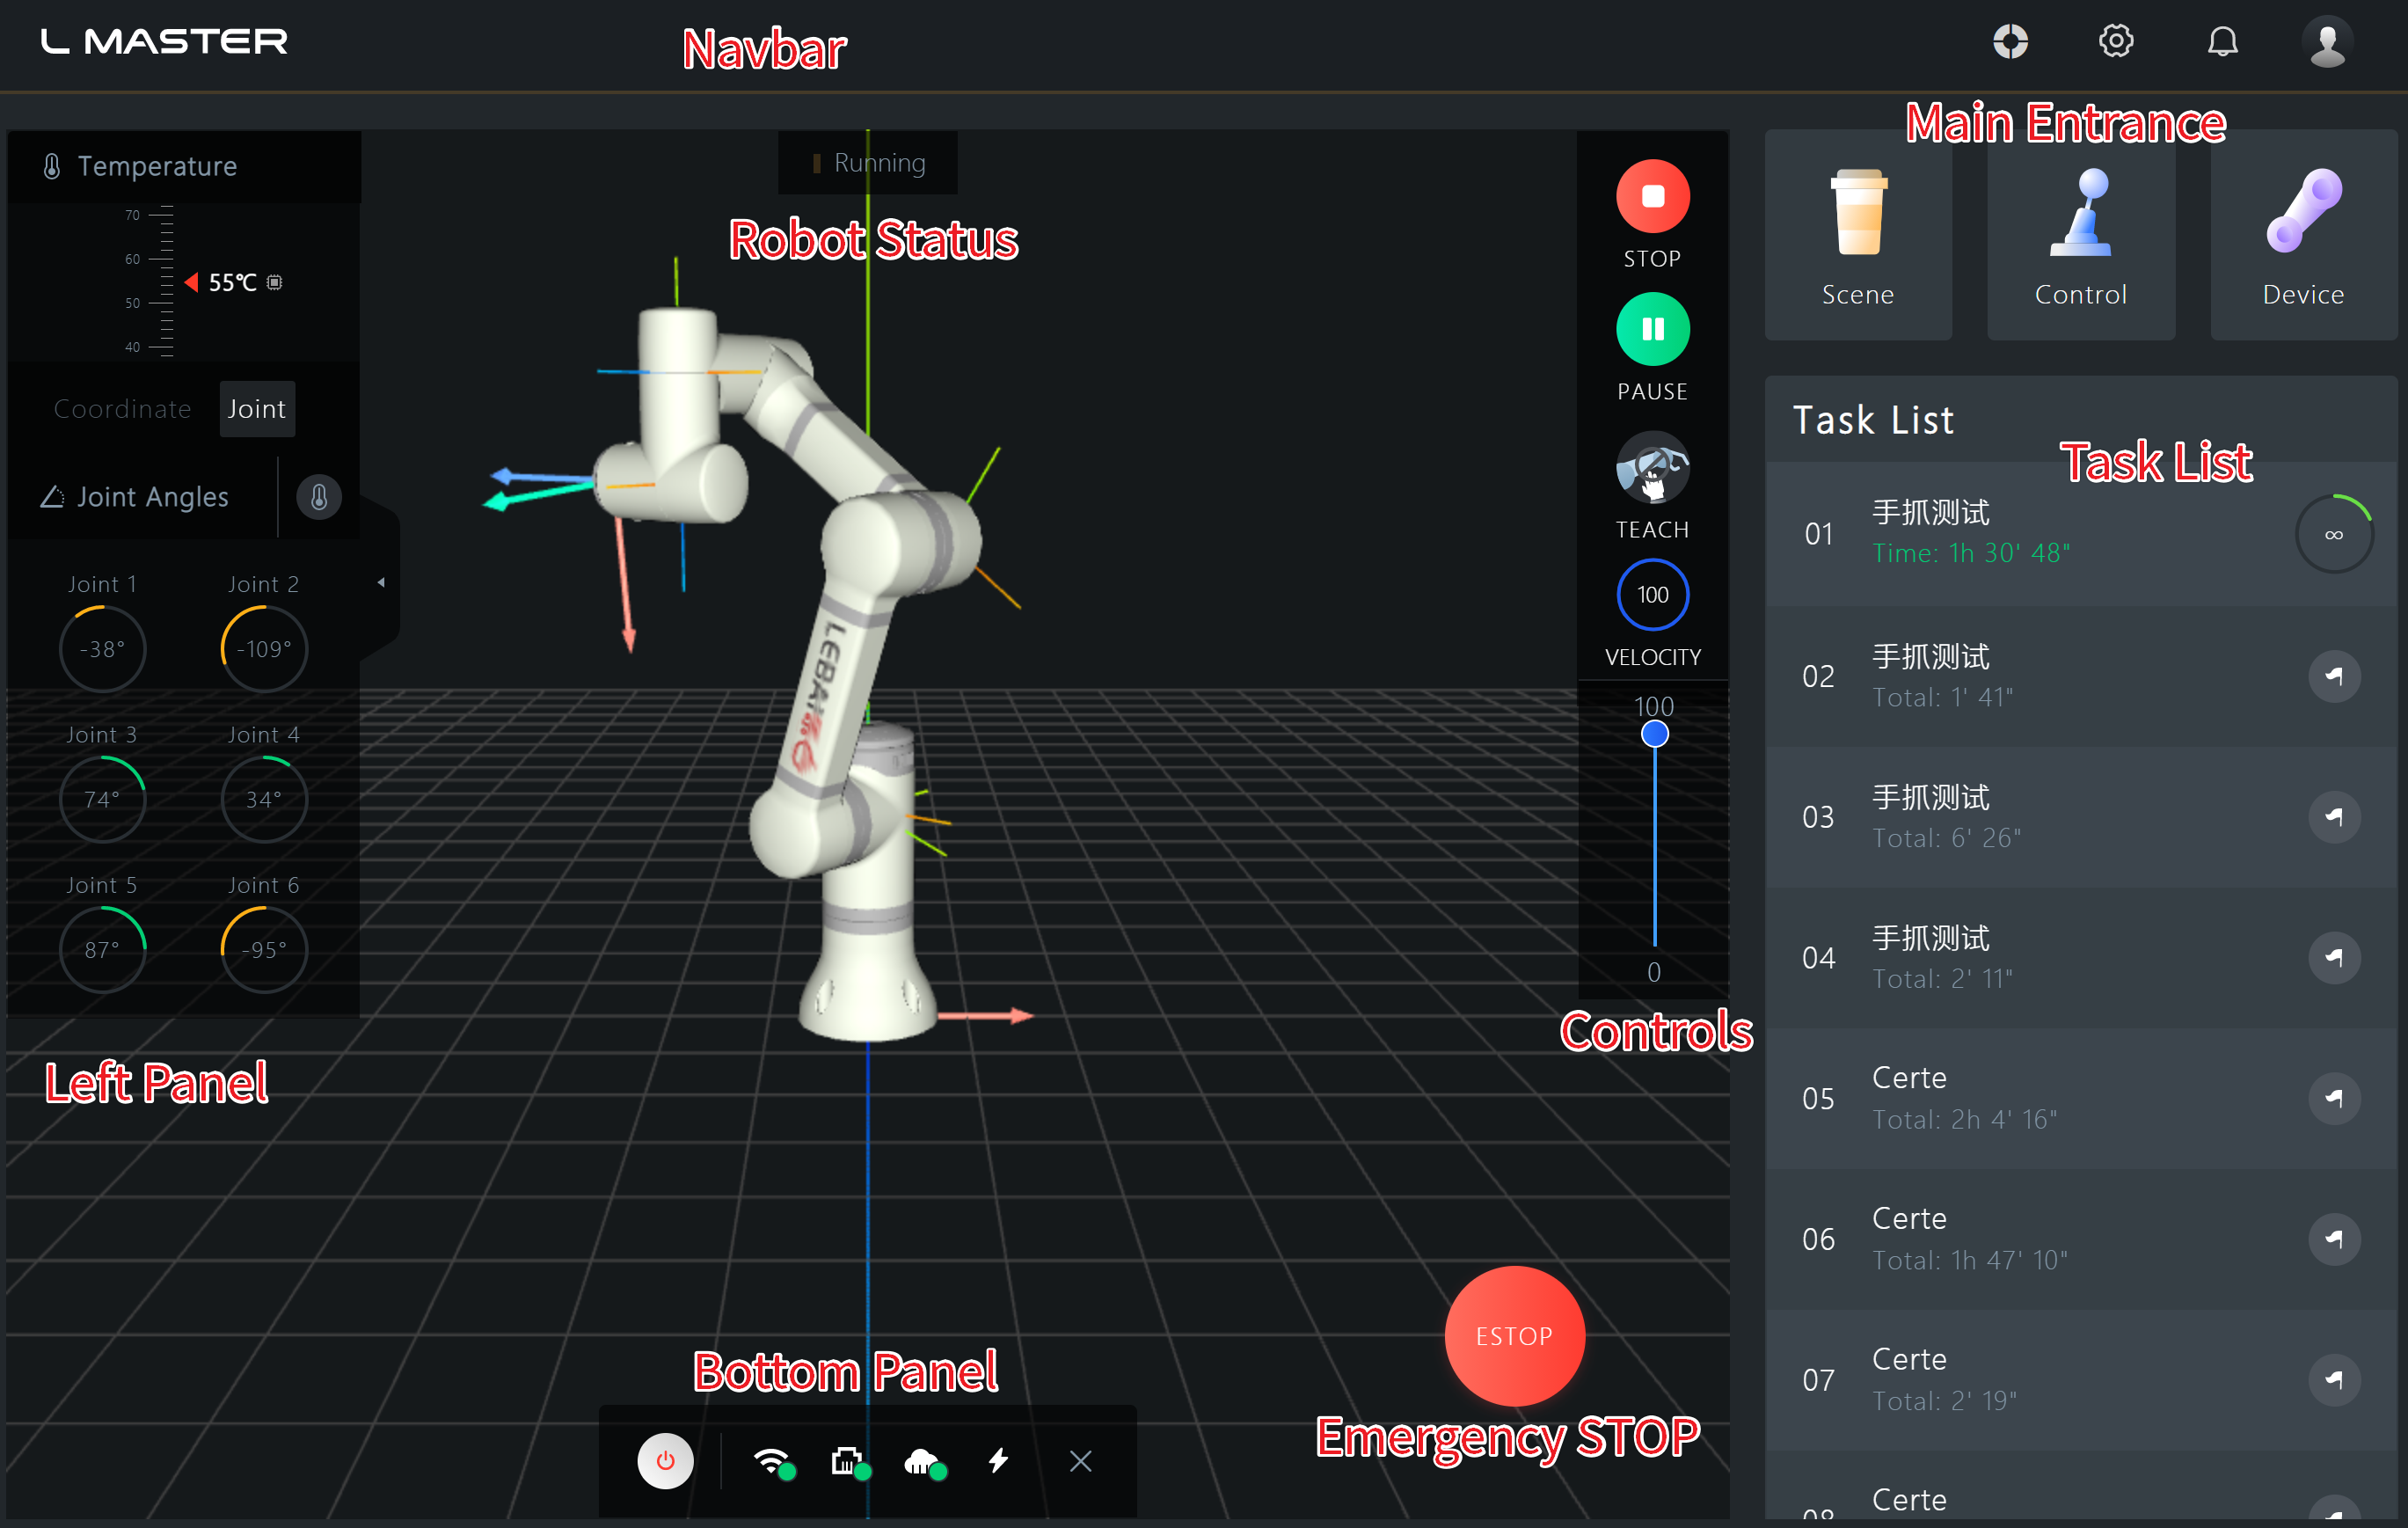
\includegraphics[width=\textwidth]{en/image/home.png}
	\caption{\LM Home}
	\label{fig:LM首页}
\end{figure}

\clearpage

\subsection{Robot Status}

The robot status area displays the current status of the robot. For details, please refer to \prettyref{tab:机器人状态列表}.

\begin{table}[ht]
    \centering\small
	\rowcolors{1}{trEven}{trOdd}
    \caption{Robot status list}
	\def\Robot{机器人}
    \begin{tabular}{cll}
\rowcolor{th} \Th{Code} & \Th{Status} & \Th{Detail}\\
-1 & System Error & Software control system exception\\
0 & Hardware Error & Hardware communication failure\\
1 & Emergency Stopped & Please confirm the safety\\
2 & Initializing & In initialization\\
4 & Initialized & Power on\\
5 & Idle & In the idle state\\
7 & Running & In operation\\
8 & Updated & System update\\
9 & Starting & Initialized to Idle process\\
10 & Stopping & The idle state goes to the stopped state\\
11 & Teaching & In teaching mode\\
12 & Stopped & In the stop state, not the emergency \\
    \end{tabular}
    \label{tab:机器人状态列表}
\end{table}

% \vspace*{-3em}
\clearpage

\subsection{Temperature Information}
As shown in \prettyref{fig:关节位置信息}, the left panel of the \LM\ homepage displays the temperature\footnote{The display of the complete machine temperature takes the maximum value of the controller CPU temperature in the control box and the temperatures of all joints of the robot. When there is a chip icon displayed on the right side of the overall temperature value, it means that the CPU has the highest temperature at the moment; when there is a joint plus number icon displayed, it means the joint corresponding to the number has the highest temperature.} of the robot in real time. The normal temperature of each joint is between room temperature and $65\oC$.
Select the \mnui{Joint} tab in the left panel, the joint angles of 6 joints are displayed by default.
Click the ~\icn{image/icon_temperature.pdf}~ icon on the right of the \mnu{Joint Angle} to observe the temperature changes of Joint 1 to Joint 6 in real time;
as shown in \prettyref{fig:温度信息}, click the \icn{image/angle.pdf} icon on the right of the \mnu{TEMPERATURES} to switch back to the joint angle display.

\begin{figure}[ht]
		\centering
		\begin{minipage}[t]{0.45\linewidth}
			\centering
			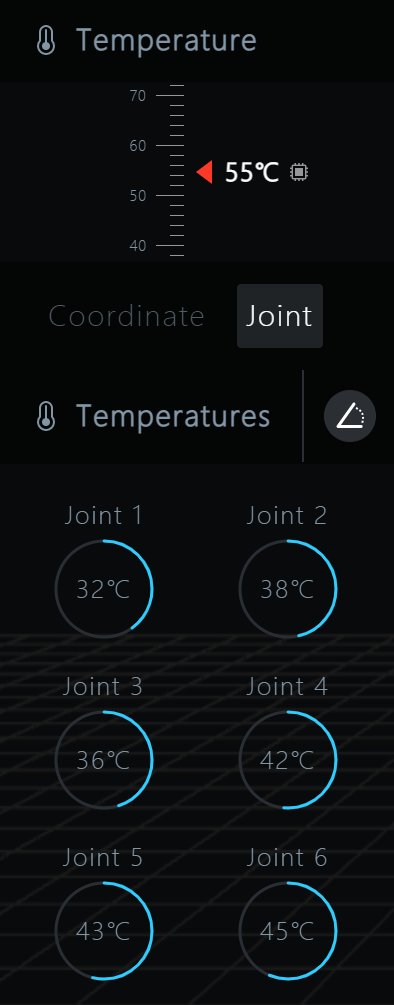
\includegraphics[height=6cm]{en/image/2-12-t.png}
			\caption{Joints' temperature}
			\label{fig:温度信息}
		\end{minipage}
		\begin{minipage}[t]{0.45\linewidth}
			\centering
			
\includegraphics[height=4cm]{en/image/2-13.png}
			\caption{Speed Ratio}
			\label{fig:速度比例}
		\end{minipage}
\end{figure}

% \vspace*{-1em}

\danger[WARNING]{When the Joint Temperature shows a value more than $65\oC$, do not touch the outer surface of the robot, otherwise there is a risk of thermal burns. Please stop the robot immediately, and check whether the current robot load exceeds the rated payload by $3\kg$ or whether the robot bumped against external objects after the temperature of the robot drops to normal.}

\begin{figure}[ht]
	\centering
	\begin{minipage}[t]{0.45\linewidth}
		\centering
		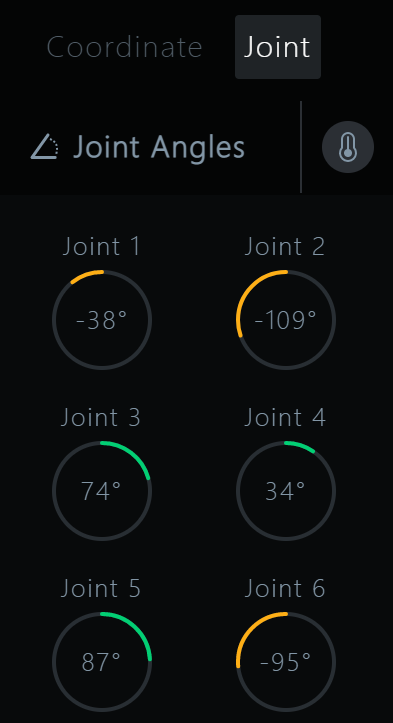
\includegraphics[height=6cm]{en/image/2-12-1.png}
		\caption{Joint space}
		\label{fig:关节位置信息}
	\end{minipage}
	\begin{minipage}[t]{0.45\linewidth}
		\centering
		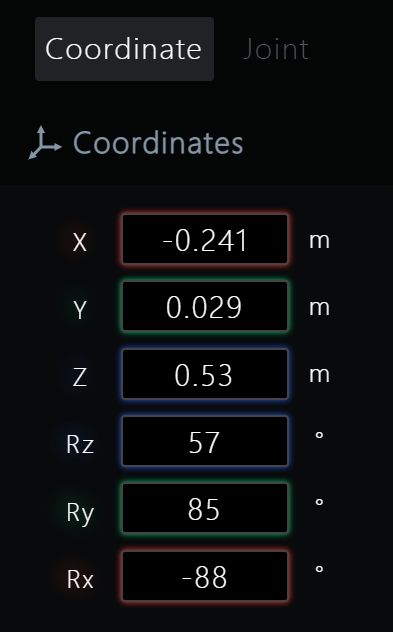
\includegraphics[height=6cm]{en/image/2-12.png}
		\caption{Coordinate space}
		\label{fig:坐标位置信息}
	\end{minipage}
\end{figure}

% \vspace*{-2em}

\subsection{Position Information}
\LM The left panel of the \LM homepage synchronizes with the position information of the robot in real time, including the Coordinate Space and Joint Space. As shown in \prettyref{fig:关节位置信息}, the Joint Space displays the real­time data of the six joint angles of the robot; as shown in \prettyref{fig:坐标位置信息}, the Coordinate Space displays the real­time data of the position and posture of the robot in the coordinate space.

\subsection{Speed Ratio}
Click the Speed icon in the control area of the \LM homepage, and drag the slider in the expanded sliding bar or click the sliding bar to adjust the robot's running speed ratio. The range of the ratio is $0\sim 100$.

% \begin{figure}[ht]
% 	\centering
% \end{figure}

\subsection{Message Center}
In the Message Center, you can view prompts, warnings, and notifications of software and hardware abnormalities of the robot.

Move the mouse to the message icon \colorbox{black}{\icn{image/22.pdf}} in the upper right corner of the \LM homepage to open the Message Center.

\begin{figure}[htb]
	\centering
	\begin{minipage}[t]{0.55\linewidth}
		\centering
		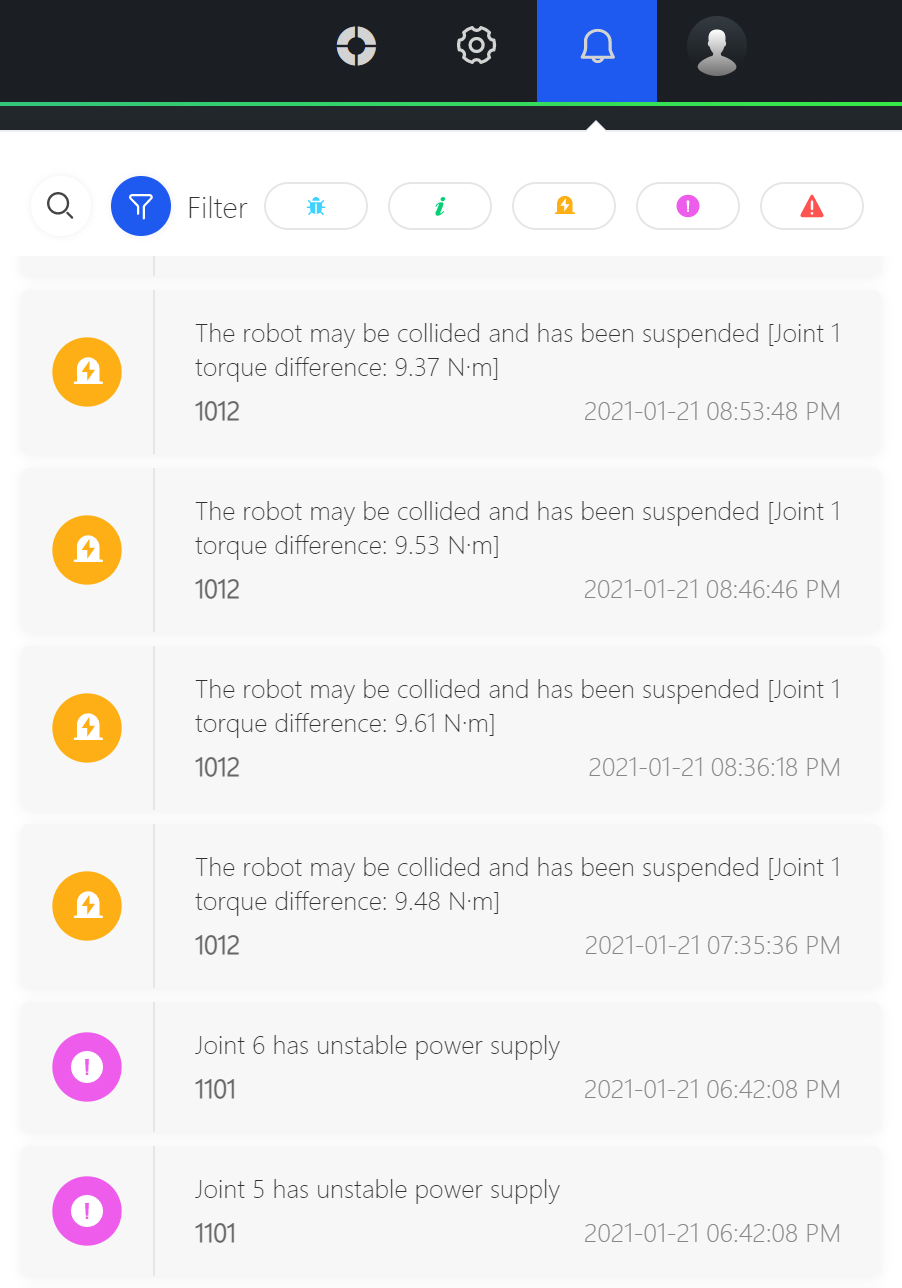
\includegraphics[height=8cm]{en/image/2-14.png}
		\caption{Message Center}
		\label{fig:消息中心}
	\end{minipage}
	\hfill
	\begin{minipage}[t]{0.4\linewidth}
		\centering
		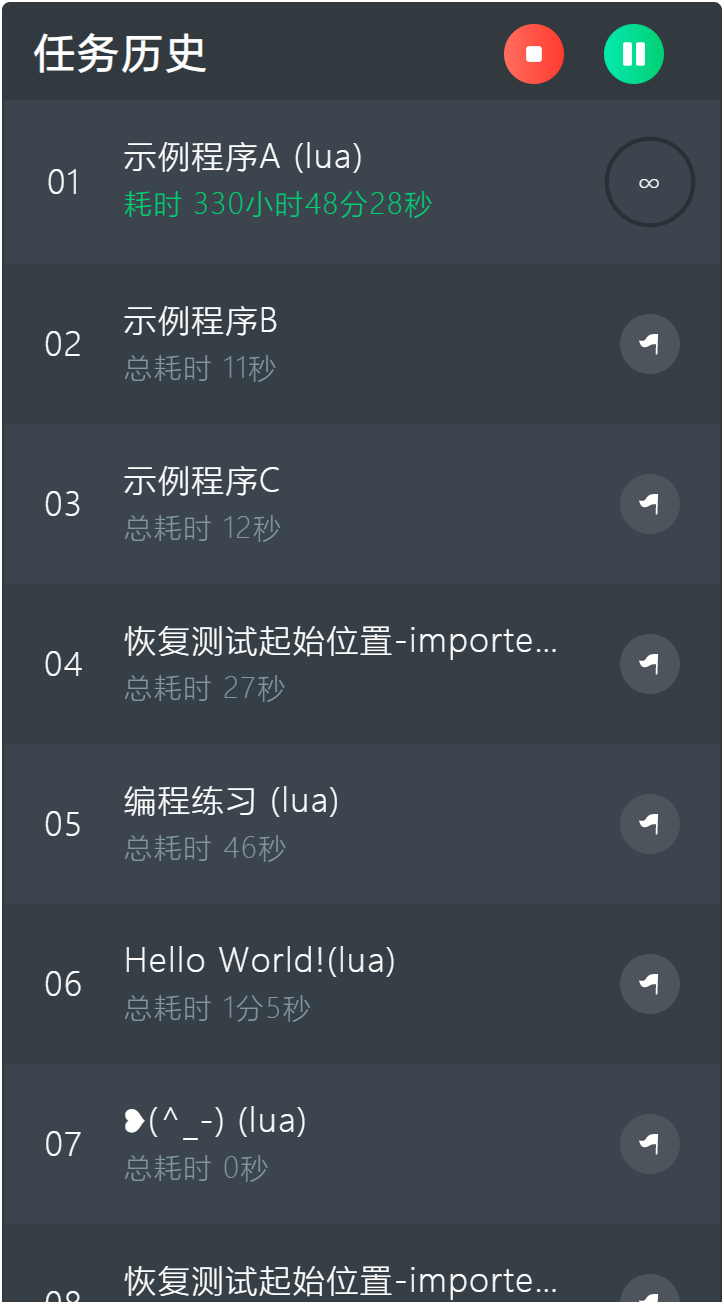
\includegraphics[height=8cm]{en/image/2-15.png}
		\caption{Task History}
		\label{fig:任务历史}
	\end{minipage}
\end{figure}
There are two ways to search for messages in Message Center,
\begin{enumerate}
	\item Search for message notifications by keywords.
	\item By filtering the following types of message notifications:
	\begin{itemize}
% \item[\icn{image/30.pdf} 调试]
\item[\icn{image/29.pdf} Info] Information reminder message.
\item[\icn{image/28.pdf} Warning] A warning level reminder during system running which generally does not affect system use.
\item[\icn{image/27.pdf} Error] There is an error in the system, and you need to pay attention to the frequency with which the error occurs. If it occurs frequently, click the error to view the solution as soon as possible or get in touch with our company in time.
\item[\icn{image/26.pdf} Fatal] The system has a severe error. There is an operational risk in the system, or the system is no longer operational. At this time, the robot must be shut down immediately. Check the solution or get in touch with our company in time.
	\end{itemize}
\end{enumerate}

As shown in \prettyref{fig:消息中心},
% 点击消息项内容左下角的错误码超链接,
the number in the lower left corner of a message is the error code. Click the error code link to jump to the corresponding error code solution page on our company's official website, where you can find the corresponding problem's explanation and solution based on the error code.

\subsection{Task History}
\label{sec:任务历史}
The task history list displays running and completed tasks in a chronological order. When a task is running, the control buttons for \mnu{STOP}, \mnu{PAUSE} or \mnu{RESUME} will appear in the task history title bar. In the task history list:
\begin{itemize}
	\item The right side of a running task displays the current number of runs and the progress of the current running cycle.
	\item The \icn{image/icon_flag.pdf}~\mnu{RERUN} button is displayed on the right side of a completed task. Click to rerun the currently selected task.
\end{itemize}

Click the task name of a task in \mnu{Task History} to enter the scene editing page corresponding to the task.

\danger[WARNING]{When running a scene, the tasks of the scene will be listed in the task history list. After a task is completed, if you click the \mnu{RERUN} button, the currently executed task will have the scene data of the previous execution of the task. Even if the scene changes after the task is completed, the re­running of the task will be unaffected. The rerun task is not affected by the data change of the scene but subject to the scene data of the last run.}

% \clearpage

\section{Start The Robot}
Enter \LM (see \prettyref{fig:启动机器人}), click the start button in the control area,after a short \mnu{STARTING}, the status area on the homepage turns to \mnu{IDLE}, indicating that you have successfully started the robot.

\begin{figure}[ht]
	\centering
	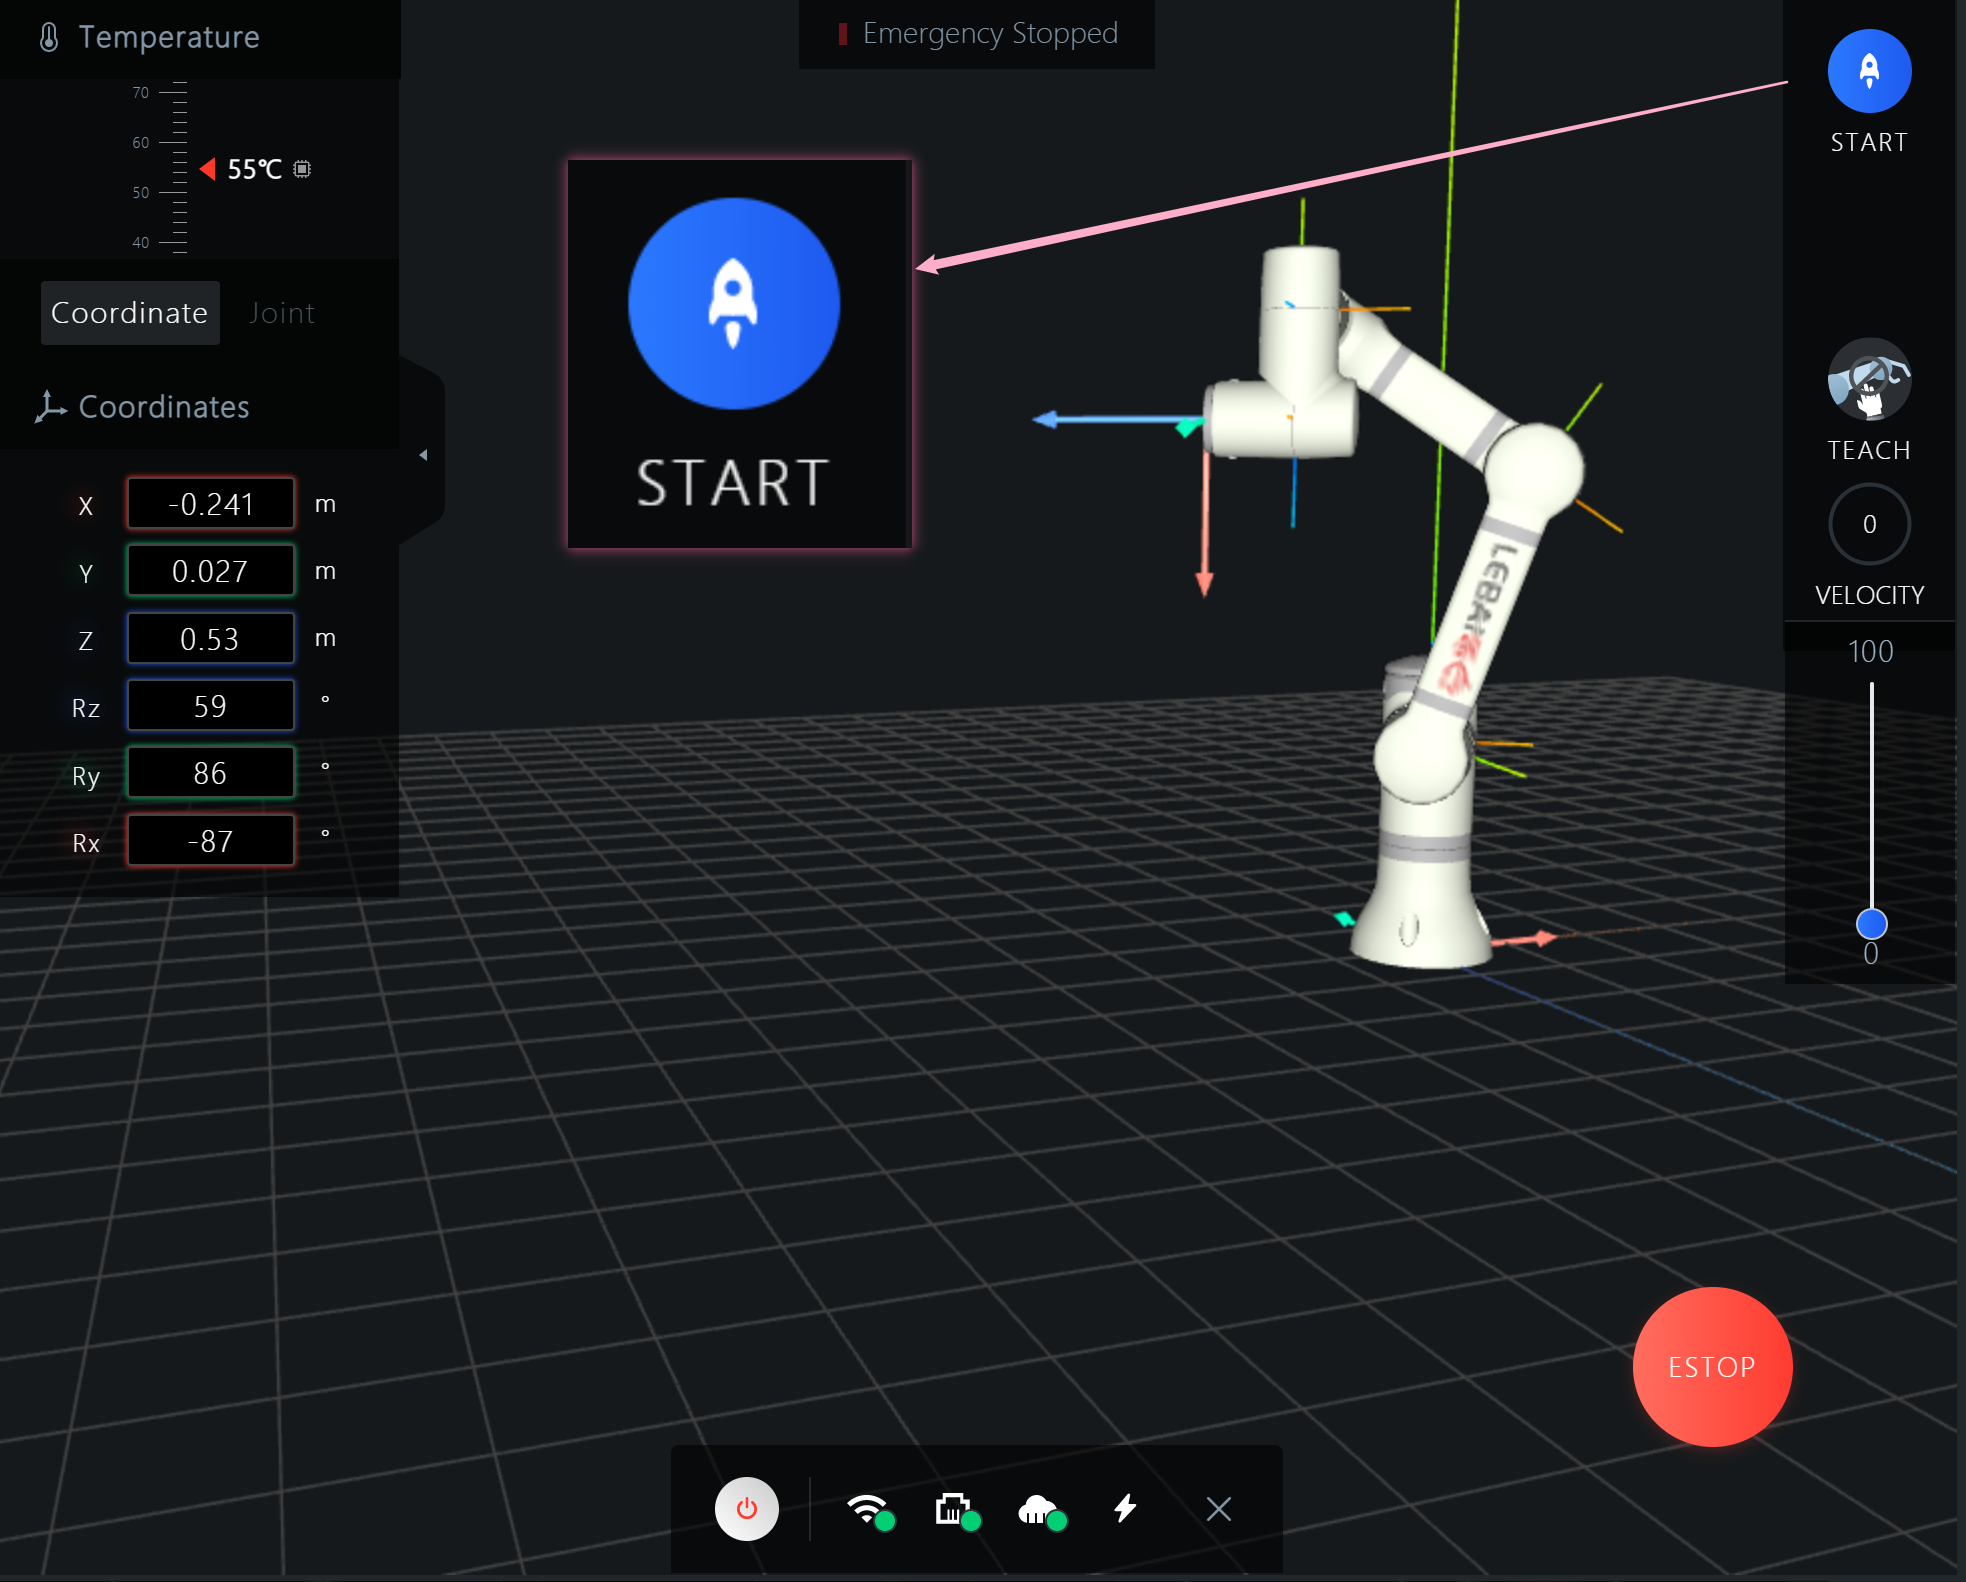
\includegraphics[width=\textwidth]{en/image/2-16.png}
	\caption{Start The Robot}
	\label{fig:启动机器人}
\end{figure}

\section{Stop The Robot}
When the robot is \mnu{RUNNING} or \mnu{IDLE}, you can click the red stop button on the homepage or in the capsule control area as shown in \prettyref{fig:胶囊控制区}. After a short \mnu{STOPPING}, when the robot status changes to \mnu{STOPPED}, it means you have successfully stopped the robot.

% \begin{figure}[ht]
% 	\centering
% 	\includegraphics[width=\textwidth]{image/6.pdf}
% 	\caption{\LM  首页--停止机器人}
% 	\label{fig:停止机器人}
% \end{figure}

\clearpage

\section{Emergency Stop}

% 急停操作有两种方式,可任选其一:
\begin{itemize}[leftmargin=3.5em]
	\item[ESTOP] The red emergency stop button at the bottom right of \LM.
	\item[Hard ESTOP] Press the emergency stop button (red raised) on the top of the control box or the external emergency stop button (optional).
\end{itemize}

\info{After using the hard emergency stop operation, the emergency stop operation will not be automatically re­ leased. You need to turn the emergency stop button clockwise to release it after unlocking.}

\section{Turn Off the Robot}
\begin{enumerate}
	\item Firstly, stop or emergency stop the robot.
	\item Long press the control box switch button or use an external switch button (optional) until the blue indicator light of the control box switch button goes out.
	\item Turn off the red main power switch on the back panel of the control box.
\end{enumerate}

\danger[WARNING]{To turn off the robot, you must strictly follow the above steps, otherwise it may cause damage to the robot's file system and malfunction of the robot.}

\section{Capsule Control}
The capsule control area is only displayed when it is not on the home page, the upper part of the capsule is the \mnu{ROBOT}, and the lower part of the capsule is the \mnu{TASK}. Long press the capsule body to drag to adjust the position of the capsule control area on the page.

\begin{figure}[hb]
	\centering
	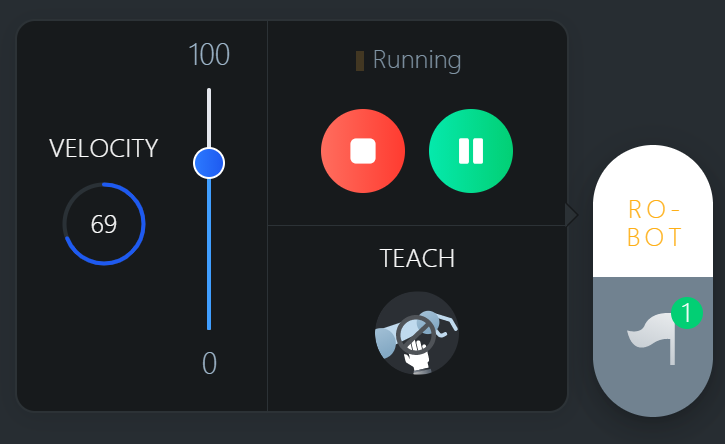
\includegraphics[height=4cm]{en/image/2-18.png}
	\caption{Capsule Control}
	\label{fig:胶囊控制区}
\end{figure}

\begin{itemize}[leftmargin=4.5em]
	\item [ROBOT] Contains the current state of the robot, the robot start/stop button, the teach button, and the speed adjustment lever. The robot can be operated and controlled when it is not on the homepage.
	\item [TASK] Contains a list of running and completed tasks and the pause/resume and stop buttons of the task. You can view the task history when it is not on the home page. For specific operations, see \prettyref{sec:任务历史}.
\end{itemize}
